\documentclass[tikz, border=12pt]{standalone}
\usepackage{tikz}
\usepackage{amsmath}
\usepackage{newtxtext, newtxmath}
\usetikzlibrary{arrows.meta, calc}

\definecolor{pumpblue}{RGB}{0,70,190}
\definecolor{pairred}{RGB}{210,40,40}
\definecolor{crystalfill}{RGB}{188,224,188}
\definecolor{projgray}{RGB}{110,110,110}

\begin{document}
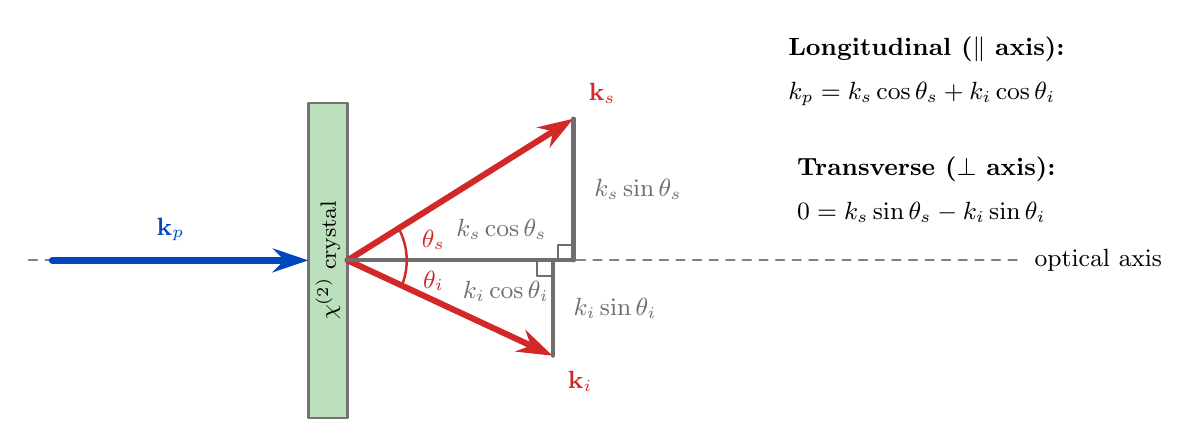
\begin{tikzpicture}[
    >=Stealth,
    line cap=round,
    line join=round,
    lbl/.style={font=\small},
]

% ── Adjustable parameters ───────────────────────────────────────────────────
\def\ths{30}    % signal angle above optical axis [degrees]
\def\thi{23}    % idler  angle below optical axis [degrees]
\def\Ls{3.6}    % length of k_s arrow
\def\Li{3.1}    % length of k_i arrow

% Crystal exit point = origin
\coordinate (O) at (0.25,0);

% Tips of signal and idler vectors
\coordinate (S) at ({\Ls*cos(\ths)},  {\Ls*sin(\ths)});
\coordinate (I) at ({\Li*cos(\thi)}, {-\Li*sin(\thi)});

% Feet of perpendiculars ON the optical axis
\coordinate (Sf) at ({\Ls*cos(\ths)},  0);   % directly below S
\coordinate (If) at ({\Li*cos(\thi)},  0);   % directly above I

% ── Optical axis ────────────────────────────────────────────────────────────
\draw[dashed, black!50, line width=0.8pt] (-3.8,0) -- (8.8,0);
\node[lbl, anchor=west] at (8.85, 0) {optical axis};

% ── Crystal slab ────────────────────────────────────────────────────────────
\filldraw[fill=crystalfill, draw=black!55, line width=0.9pt]
    (-0.25,-2) rectangle (0.25,2);
\node[font=\footnotesize, align=center, rotate=90] at (0,0)
    {$\chi^{(2)}$ crystal};

% ── Pump arrow ──────────────────────────────────────────────────────────────
\draw[-{Stealth[length=4.5mm,width=3mm]}, line width=2.6pt, pumpblue]
    (-3.5,0) -- (-0.25,0);
\node[lbl, pumpblue, above] at (-2.0, 0.12) {$\mathbf{k}_p$};

% ── Signal vector ───────────────────────────────────────────────────────────
\draw[-{Stealth[length=4.5mm,width=3mm]}, line width=2.2pt, pairred]
    (O) -- (S);
\node[lbl, pairred, above right=2pt] at (S) {$\mathbf{k}_s$};

% ── Idler vector ────────────────────────────────────────────────────────────
\draw[-{Stealth[length=4.5mm,width=3mm]}, line width=2.2pt, pairred]
    (O) -- (I);
\node[lbl, pairred, below right=2pt] at (I) {$\mathbf{k}_i$};

% ── Signal right triangle ───────────────────────────────────────────────────
% Horizontal leg: O --> Sf  (on the axis)
\draw[projgray, line width=1.5pt] (O) -- (Sf);
% Vertical leg: Sf --> S  (perpendicular to axis)
\draw[projgray, line width=1.5pt] (Sf) -- (S);
% Right-angle box at Sf
\draw[projgray, line width=0.75pt]
    ($(Sf)+(0, 0.20)$) -- ($(Sf)+(-0.20, 0.20)$) -- ($(Sf)+(-0.20, 0)$);
% Component labels
\node[lbl, projgray, below=4pt] at ($(O)!0.7!(Sf)$)
    {$k_i\cos\theta_i$};
\node[lbl, projgray, right=4pt] at ($(Sf)!0.5!(S)$)
    {$k_s\sin\theta_s$};

% ── Idler right triangle ────────────────────────────────────────────────────
% Horizontal leg: O --> If  (on the axis)
\draw[projgray, line width=1.5pt] (O) -- (If);
% Vertical leg: If --> I  (perpendicular to axis, going downward)
\draw[projgray, line width=1.5pt] (If) -- (I);
% Right-angle box at If
\draw[projgray, line width=0.75pt]
    ($(If)+(0,-0.20)$) -- ($(If)+(-0.20,-0.20)$) -- ($(If)+(-0.20, 0)$);

% Component labels
\node[lbl, projgray, above=4pt] at ($(O)!0.75!(If)$)
    {$k_s\cos\theta_s$};
\node[lbl, projgray, right=4pt] at ($(If)!0.5!(I)$)
    {$k_i\sin\theta_i$};

% ── Angle arcs ──────────────────────────────────────────────────────────────
\draw[pairred, line width=0.9pt]
    (1,0) arc[start angle=0, end angle=\ths, radius=0.85];
\node[pairred, lbl] at (1.34, 0.26) {$\theta_s$};

\draw[pairred, line width=0.9pt]
    (1,0) arc[start angle=0, end angle=-\thi, radius=0.85];
\node[pairred, lbl] at (1.34,-0.26) {$\theta_i$};

% ── Conservation equations ──────────────────────────────────────────────────
\node[align=left, font=\small] at (7.6, 2.4) {
    \textbf{Longitudinal ($\parallel$ axis):}\\[5pt]
    $k_p = k_s\cos\theta_s + k_i\cos\theta_i$
};
\node[align=left, font=\small] at (7.6, 0.9) {
    \textbf{Transverse ($\perp$ axis):}\\[5pt]
    $0 = k_s\sin\theta_s - k_i\sin\theta_i$
};

\end{tikzpicture}
\end{document}